\documentclass[a4paper]{book}

% packages % 
\usepackage[utf8]{inputenc} 
\usepackage{fvextra}
\usepackage{csquotes}
\usepackage[french, italian, spanish, english]{babel}
\usepackage[T1]{fontenc}   
\usepackage{color}  
\usepackage{amsmath, dsfont, amssymb, amsthm, stmaryrd}
\usepackage[style=alphabetic]{biblatex}
\usepackage{enumitem}
\usepackage[hidelinks]{hyperref}

% graphics %
\usepackage{graphicx}
\graphicspath{ {./images/} }

% environments %
\newtheorem{theorem}{Theorem}[section]
\newtheorem{corollary}{Corollary}[theorem]
\newtheorem{lemma}[theorem]{Lemma}

\theoremstyle{definition}
\newtheorem{definition}{Definition}[section]

\theoremstyle{remark}
\newtheorem*{remark}{Remark}
\newtheorem*{example}{Example}



% bibliography %
\bibliography{bibliography} 

\begin{document}

% title %
\title{General Relativity}
\author{Buisine Léo\\Ecole Normale Superieure of Paris}
\maketitle

\tableofcontents

\chapter{Introduction}
Danièle Steer: daniele.steer@phys.ens.fr \newline
work on theories of gravity, gravitational waves, primordial cosmology \par \medskip 

We should do the TD before the TD. \par \medskip 

This will be a course more physical than mathematical. No differential geometry or Cartan geometry. The TD will be more formal. The objective is to understand current experiments and current measures. As such, we will mostly stay outside of black holes horizons. We will also use cevtors in coordinate basis. We should remember that physics is independant of the choice of coordinates. The objective is to be able to do accurate computations.\par \bigskip 

Aims:
\begin{enumerate}
    \item Handle GR and its tools
    \item Be able to do accurate calculations 
    \item Have a feeling for different works in GR today
\end{enumerate} \bigskip 

The current GR fails at cosmological scale. It doesn't explain the Hubble constant, Dark energy nor Dark matter. Many theories try to modify GR, but many of these modified gravities are constantly ruled out by new experiments and new data. For exemple, a whole lot of theories were ruled out in 2017 by an experiment showing that 
\begin{equation}
    \left|\frac{c_{GW}-c}{c}\right| < 10^{-15}
\end{equation}\par \medskip 

The Newtonian gravity potential on the surface of a body of mass $M$ and radius $R$ is given by 
\begin{equation}
    \Phi_N = \frac{GM}{R}
\end{equation}
The Newtonian gravity is valid in the limit $\Phi_N << 1$. 
\begin{enumerate}
    \item On earth, we have $\Phi_N \sim 10^-9$
    \item On the sun, we have $\Phi_N \sim 10^-6$
    \item On a neutron star, we have $\Phi_N \sim 10^-1$
    \item In a black hole, there is no upper limit
\end{enumerate}\bigskip \par \medskip 

Semi classical gravity is doing QFT in curved spacetime. The idea is to start with a classical solution of Einstein's equation. Then we quantise the field in this metric. Then we can loop, compute the change in the metric due to the field, then re quantise the field, etc... The result of this computation gives the famous Hawking temperature of black holes 
\begin{equation}
    T_H = \frac{hbarc^3}{8\pi GMk_B}
\end{equation}
For a BH of mass of the sun $M_\Theta$, $T_H \sim 10^{-8}$K. This causes the decay of black holes such as primordial black holes.\par \medskip 

GR is a very unique theory. Therem of lovelock (1972): Einstein's equations are the unique 2nd order local equation of motion for a metric $g_{\mu\nu}$ derivable from an action in 4D. \par 

So if we want to go beyond GR, we can either work in more than 4D, add extra fields (ex scalar-tensor theories of gravity), we can try higher order equations of motion, or we can remove the locality. 
\chapter{Overview}
\section{Special Relativity}

For our Minkowski metric, we will take the signature $(-, +, +, +)$. SR describes all forces apart from gravity, and they live on a fixed Minkowski spacetime. \par \medskip 

In SR, there is a class of globally defined non-accelerating inertial observers, with associated pseudo-cartesian coords 
\begin{equation}
    x^\mu = (ct, x, y, z) \qquad \eta_{\mu\nu} = \text{diag}(-1, 1, 1, 1)
\end{equation}
IN GR, gravitational force is a manifestation of curvature $\eta_{\mu\nu} \rightarrow g_{\mu\nu}(x)$, given by Einstein's equation 
\begin{equation}
    G_{\mu\nu} = \frac{8\pi G}{c^4}T_{\mu\nu}
\end{equation}
We have $\frac{8\pi G}{c^4} \sim 10^{43}$. $G_{\mu\nu}$ is intrisicly related to the curvature of spacetime, by the RIemann tensor for exemple. It has dimension inverse length square? $T_{\mu\nu}$ is the energy-momentum tensor. \par \medskip 

We have 2nd order non-linear PDE for $g_{\mu\nu}(x)$. To find the solutions, we can impose symmetries 

\begin{enumerate}
    \item Cylinder symmetry: string-like BH
    \item Time independant spherical symmetry: Schwarchild BH 
    \item Planar symmetry: Domorin-Wall cosmological solution in 5D, it is a modified gravity theory
\end{enumerate}

Another idea is to do perturbative physics, and to find perturbative solutions. 
\begin{equation}
    g_{\mu\nu}(x) = \bar{g}_{\mu\nu}(x) + \delta g_{\mu\nu}(x)
\end{equation}
$\bar{g}_{\mu\nu}$ is a known solution, but can be a lot of things. Either Minkowski spacetime, either Schwarchild blackhole, either FRWL, ... \par \medskip 

Another possibility to solve the equations is when $\Phi_N << 1$, where we have 
\begin{equation}
    \nabla ^2 \Phi = 4\pi G\rho  
\end{equation}
with $\rho$ the mass density. \par \medskip 

Geodesic equation for test masses, subject only to gravity. 
\begin{equation}
    \frac{\text{d}^2x^\mu}{\text{d}\lambda^2} + \Gamma^\mu_{\alpha\beta} \frac{\text{d}x^\alpha}{\text{d}\lambda} \frac{\text{d} x^\beta}{\text{d}\lambda} = 0
\end{equation}
equation for $x^\mu(\lambda)$, the world line of the test mass $(m>0)$, where $\lambda$ is the time perceived by the body following the geodesic, an (often, but not always: see 1st TD) affine parameter of the proper time. \par \medskip 

The Christoffel symbol is given by 
\begin{equation}
    \Gamma^\mu_{\alpha\beta} = \frac{1}{2}g^{\mu\nu} (\partial_\alpha g_{\nu\beta} + \partial_\beta g_{\nu\alpha} - \partial_\nu g_{\alpha\beta})
\end{equation}\par \medskip 

In the limit $\Phi_N << 1$, it reduces to $\vec{a} = - \vec{\nabla} \Phi_N$. This is independant of the composition of the particle (universal equation). It is a consequence of $m_i = m_g$. THe current experiments say that 
\begin{equation*}
    \left|\frac{m_i - m_g}{m_g}\right| \sim 10^{-15}
\end{equation*}
Weak equivalence principle: $m_i = m_g$. \par \medskip 

In GR, a consequence of the WEP is that locally, gravity and acceleration are indistinguishable. Locally, the effect of gravity can be removed by going to a locally freely falling frame (LFFF).\par 
Einstein's EP: in the LFFF, the laws of physics are those of SR. Locally, $g_{\mu\nu} \sim \eta_{\mu\nu}$. 

\section{Rindler's space}

A few work on SR and Rindler Space
\begin{itemize}
    \item $x^\mu = (t, x, y, z)$ associate to globally defined non accelerating inertial observer 
    \item $\eta_{\mu\nu} = \text{diag}(-, +, +, +)$
    \item different inertial frames related by Lorentz transformations $x'^\mu = \Lambda ^\mu_\nu x^\nu$
    \item Free massive particles satisfy $\frac{\text{d}^2x^\mu}{\text{d}\tau^2} = 0$ where $\tau$ is the proper time, $ds^2 = -d\tau^2$
\end{itemize}

Now let's work in general curvilinear coords 
\begin{equation}
    x^\mu \rightarrow y^\mu(x^\alpha) \text{(assumed invertible)}
\end{equation}
\begin{example}
    spherical polar coords $y^\alpha = (t, r, \theta, \phi)$
\end{example}
\begin{example}
    Rindler: $y^\alpha = (\eta, \rho, y, z)$
\end{example}
\underline{Metric}: 
\begin{equation}
    ds^2 = \eta_{\mu\nu} \text{d}x^\mu \text{d}x^\nu = \eta _{\mu\nu} \frac{\partial x^\mu}{\partial y ^\alpha} \frac{\partial x^\nu}{\partial y ^\beta} \text{d} y^\alpha \text{d}y ^\beta
\end{equation}
with 
\begin{equation}
    \eta _{\mu\nu} \frac{\partial x^\mu}{\partial y ^\alpha} \frac{\partial x^\nu}{\partial y ^\beta}  = g_{\alpha\beta}(y)
\end{equation}
The inverse is 
\begin{equation}
    g^{\alpha\beta} = \eta ^{\mu\nu} \frac{\partial y ^\alpha}{\partial x^\mu} \frac{\partial y ^\beta}{\partial x^\nu} 
\end{equation}
Check 
\begin{equation}
    g^{\alpha\beta}g_{\beta\gamma} = \delta^\alpha_\gamma
\end{equation}

In the new coord system, $\frac{\text{d}^2x^\mu}{\text{d}\tau^2} = 0$. So 
\begin{equation}
    \frac{\text{d}^2y^\mu}{\text{d} \tau^2} + \tilde{\Gamma}^\mu_{\alpha\beta}\frac{\text{d}y^\alpha}{\text{d}\tau}\frac{\text{d}y^\beta}{\text{d}\tau} = 0
\end{equation}
where 
\begin{equation}
    \tilde{\Gamma}^\mu_{\alpha\beta} = \frac{\partial y^\mu}{\partial x^\omega} \frac{\partial^2 x^\omega}{\partial y^\alpha\partial y^\beta } = \frac{1}{2}g^{\mu\epsilon}(\partial_\alpha g_{\epsilon\beta} + \partial_\beta g_{\epsilon\alpha} - \partial_\epsilon g_{\alpha\beta})
\end{equation}
Geodesic equation, but note that we are in flat spacetime!\par \medskip 

Now consider a particular class of non-inertial observers, namely one with constant eternal proper acceleration along $x$ axis $1/r_0$ with $r_0 > 0$. (this is very unphysical). 
\begin{figure}
    \centering
    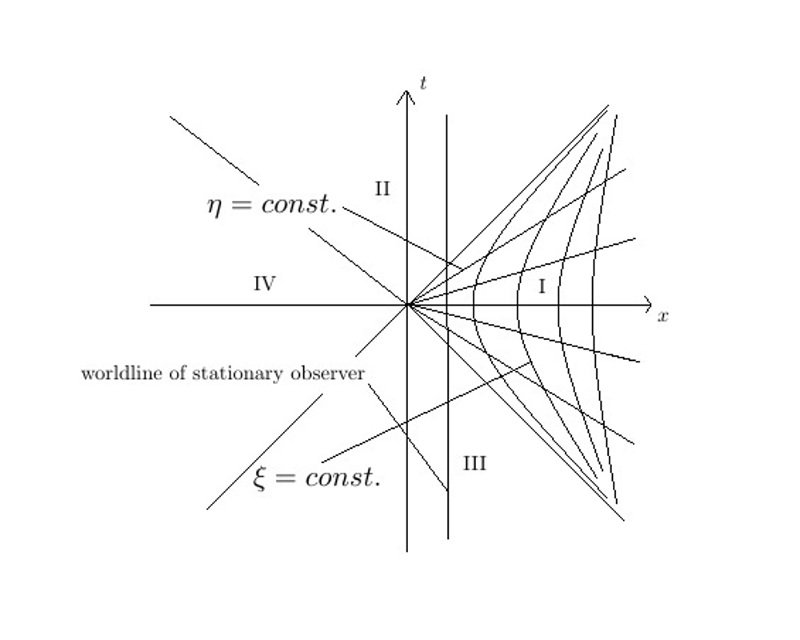
\includegraphics[width=0.7\textwidth]{rindler_coords}
    \caption{Rindler's observers}
\end{figure}
\begin{equation}
    A^\mu A_\mu = \text{const} = 1/r_0^2
\end{equation}
\begin{equation}
    A^\mu = \frac{\text{d} u^\mu}{\text{d}\tau}, \qquad u^\mu = \frac{\text{d}x^\mu}{\text{d}\tau} = (\gamma, \gamma v, 0, 0)
\end{equation}
where 
\begin{equation}
    \gamma = \frac{1}{\sqrt{1-v^2}} \quad v = \frac{\text{d}x}{\text{d}t} \quad a = \frac{\text{d}v}{\text{d}t}
\end{equation}

We can send these Rindler observers in space, resulting in the trajectories 
\begin{equation}
    \begin{aligned}
        &t = r_0 ~ \text{sinh}(\eta)\\
        &x = r_0 ~ \text{cosh}(\eta)
    \end{aligned}
\end{equation}
with $\eta = \tau/r_0$

The Rindler space is the space occupied by the trajectory of the Rindler observers, corresponding to the right wedge of the Minkowski spacetime. \par \medskip 
This allows us to parametrize the right wedge of the Minkowski spacetime, as 
\begin{equation}
   \begin{aligned}
    &t = \rho ~ \text{sinh}(\eta) \\
    &x = \rho ~ \text{cosh}(\eta)
   \end{aligned}
\end{equation}
These give the Kindler coordinates $(\rho, \eta, y, z)$ with $\rho > 0$ and $-\infty < \eta < + \infty$. In these coords, 
\begin{equation}
    \text{d}s^2 = -\rho^2 \text{d}\eta^2 + \text{d}\rho ^2 + \text{d}y^2 + \text{d}z^2
\end{equation}
Sometimes, we write $\rho = e^\chi$ in which case 
\begin{equation}
    \text{d}s^2 = e^{2\chi}\left(-\text{d}\eta^2 + \text{d}\chi^2 \right) + \text{d}y^2 + \text{d}z^2
\end{equation}\bigskip 

Now, let's look at the Schwarchild metric. For $r > r_s$
\begin{equation}
    \text{d}s^2 = -\left(1-\frac{r_s}{r}\right)\text{d}t^2 + \frac{1}{(1-\frac{r_s}{r})}\text{d}r^2 + r^2\text{d}\Omega^2
\end{equation}
where $r_s = 2GM$ and 
\begin{equation}
    \text{d}\Omega^2 = \text{d}\theta^2 + \sin^2(\theta) \text{d}\phi^2
\end{equation}
We want to consider the Schwarchild metric very near the BH horizon. We expand at first order $r = r_s + \varepsilon$
\begin{equation}
    \text{d}s^2 = -\frac{\varepsilon}{r_s}\text{d}t^2 + \frac{r_s}{\varepsilon}\text{d}\varepsilon^2 + r_s^2\text{d}\Omega^2
\end{equation}
Let 
\begin{equation}
    \begin{aligned}
        &\rho = 2\sqrt{r_s\varepsilon}\\
        & \text{d}\rho = \sqrt{\frac{r_s}{\varepsilon}}\text{d}\varepsilon
    \end{aligned}
\end{equation}
We have 
\begin{equation}
    \text{d}s^2 = -\frac{\rho^2}{4r_s^2}\text{d}t^2 + \text{d}\rho^2 + r_s^2\text{d}\Omega^2
\end{equation}
So with 
\begin{equation}
    \eta = \frac{t}{2r_s}
\end{equation}
We get 
\begin{equation}
    \text{d}s^2 = -\rho^2\text{d}\eta^2 + \text{d}\rho^2 + r_s^2\text{d}\Omega^2
\end{equation}
Which is, for the particular part, exactly the Rindler metric. So the Rindler space modelizes at first order the exterior near horizon of a black hole.

\chapter{Formalism}

GR is based on 4 postulates 
\begin{enumerate}
    \item Spacetime is 4D Lorentzian manifold, equipped with a Levi-Civita connexion $(\Gamma^\mu_{\alpha\beta})$
    \item Free particles follow time-like or null geodesics $(m > 0, \quad m = 0)$
    \item The energy, momentum and stresses of matter are described by a symmetric tensor $T_{\mu\nu}$, which is covariantly conserved $\nabla^\mu T_{\mu\nu} = 0$
    \item The curvature of space time is related to $T_{\mu\nu}$ via the Einstein's equation $G_{\mu\nu} = \frac{8\pi G}{c^4}T_{\mu\nu}$
\end{enumerate}

\underline{Differentiable manifold, scalars, vectors, tensors, forms}
\begin{enumerate}
    \item In GR, space time has a curved geometry; in general no particular symmetry and hence no preferred set of coords 
    \item Furthermore, a single set of coords is not always sufficient to describe all of spacetime (ex. Schwarchild)
    \item Manifold structure gives us the framework for smoothly meshing these coordinates together; and that any point $p$ on $\mathcal{M}$ can be thought in term of curvilinear coordinates on $\mathbb{R}^n$ (if $\mathcal{M}$ has dimension $n$)
    \begin{equation}
        \begin{aligned}
            &x(p) = (x^1(p), x^2(p), \dots, x^n(p)) \\
            &x'(p) = (x^{'1}(p), x^{'2}(p), \dots, x^{'n}(p)) 
        \end{aligned}
    \end{equation}
    and the map between $x$ and $x'$ is smooth and invertible
    \item  Scalars are invariant under coord transformations 
    \item vectors are abstractly $(\bar{x} = x^\mu\partial_\mu)$, but we will think of them as $(x^\mu)$. They are defined on the tangent space $T_p$ at point $p$, for which a natural coordinate basis is $\partial_\mu \equiv \frac{\partial}{\partial x^\mu}$. $\bar{x}$ is invariant under coordinate transformations. Thus, under the change $x \rightarrow x'$, we have 
    \begin{equation}
        x^{'\mu}(x) = \frac{\partial x^{'\mu}}{\partial x^\alpha} x^\alpha(x)
    \end{equation}
    \item covectors have as natural coord basis $\text{d}x^\mu$; $\omega = \omega_\mu \text{d}x^\mu$. We have under the transformation of coordinate 
    \begin{equation}
        \omega_\mu'(x) = \frac{\partial x^\alpha}{\partial x^{'\mu}}\omega_\alpha(x)
    \end{equation}
    \item $(k, l)$ tensors transform as $k$ vectors and $l$ covectors. 
    \item Principle of covariance: physical laws must be the same for all observers whatever their coord system. They must preserve their form under general coord transformations. For exemple, the equation for geodesics is invariant under coordinate systems 
    \begin{equation}
        \frac{\text{d}^2x^\mu}{\text{d}\tau^2} + \Gamma^\mu_{\alpha\beta} \frac{\text{d}x^\alpha}{\text{d}\tau}\frac{\text{d}x^\beta}{\text{d}\tau} = 0
    \end{equation}
    Writing it out gives us the transformation law of $\Gamma$. We find 
    \begin{equation}
        \Gamma{'\nu}_{\alpha\beta} = \frac{\partial x^{'\nu}}{\partial x^{\omega}}\frac{\partial x^{\mu}}{\partial x^{'\alpha}}\frac{\partial x^{\lambda}}{\partial x^{'\beta}}\Gamma{'\omega}_{\mu\lambda} + \frac{\partial x^{\mu}}{\partial x^{'\alpha}}\frac{\partial x^{\lambda}}{\partial x^{'\beta}} \frac{\partial^2 x^{'\nu}}{\partial x^\mu \partial x^{\lambda}}
    \end{equation}
    In particular, $\Gamma$ is not a tensor. 
\end{enumerate}

\section{(Anti-) symmetrisation of tensors}. \newline 
Given some tensor $B_{\mu\nu}$, we can symmetrize it by taking 
\begin{equation}
    S_{\mu\nu} = \frac{1}{2}(B_{\mu\nu} + B_{\nu\mu})
\end{equation}
we can antisymmetrize it by taking 
\begin{equation}
    A_{\mu\nu} = \frac{1}{2}(B_{\mu\nu} - B_{\nu\mu})
\end{equation}
For a tensor with $n$ indices, we consider permutations, and we have 
\begin{equation}
    T_{(\mu_1, \dots, \mu_n)} = \frac{1}{n!}\sum_{\text{perm }\sigma} T_{\sigma(\mu_1), \dots, \sigma(\mu_n)} \qquad T_{[\mu_1, \dots, \mu_n]} = \frac{1}{n!}\sum_{\text{perm }\sigma} \text{sign}(\sigma) T_{\sigma(\mu_1), \dots, \sigma(\mu_n)} \qquad 
\end{equation}
where we write a tensor with indices in $()$ for a symmetrized tensor, and in $[]$ for an antisymmetrized tensor. \par \medskip 

By convention, we write 
\begin{equation}
    T^{(\mu_1 \mu_2)}_{\qquad[\mu_3, \mu_4](\mu_5|\mu_6|\mu_7)}
\end{equation}
a tensor symmetric in $\mu_1 \leftrightarrow \mu_2$ and in $\mu_5 \leftrightarrow \mu_7$, and antisymmetric in $\mu_3 \leftrightarrow \mu_4$ \par \bigskip 

\section{Derivatives}
Since we haven't introduced a metric, we only have $\partial_\mu$.
\begin{enumerate}
    \item $\partial_\mu f$ transforms like a vector 
    \item $\partial_\mu A^\nu$ does not transform as a $(1, 1)$ tensor 
\end{enumerate}
there is a class of tensors for which $\partial_\mu$ does take tensors to $(k, l+1)$ tensors. These are totally antisymmetric $(0, p)$ tensors $\omega_{\mu_1, \dots \mu_p} = \omega_{[\mu_1, \dots \mu_p]}$ known as $p$-forms. In dimension $n$, there are $\binom{n}{p}$ independant functions in a $p$-forms. \par \medskip 
The exterior derivative $\text{d}$ takes a $p$-form to a $(p+1)$-form 
\begin{equation}
    (\text{d}A)_{\mu_1,\dots,\mu_{p+1}} = (p+1)\partial_{[\mu_1}A_{\mu_2, \dots, \mu_{p+1}]}
\end{equation}
$\text{d}A$ is a tensor. Also, $\text{d}^2 = 0$. GR cannot be only formulated in term of forms. 

\section{Metric and tensor densities}
\begin{enumerate}
    \item Metric gives a notion of distance on the manifold 
    \item $(0, 2)$ symmetric tensor $g_{\mu\nu} = g_{\nu\mu}$
    \item non degenerate $g \equiv \det(g_{\mu\nu}) \neq 0$ (the det is not a scalar, it changes under coord transforms)
    \item $g_{\mu\nu}$ can be diagonalized, diag elements are non-zero. We can rescale basis vectors, so the values are $\pm1$. Lorentzian manifolds have signature $(-+++\dots)$ 
    \item Inverse metric $g^{\mu\nu}$ such that $g^{\mu\nu}g_{\nu\alpha} = \delta^\mu_\alpha$
    \item Metric and inverse, raise and lower indices 
    \item $A^\mu = g^{\mu\nu}A_\nu$
    \item The distance between two space time points is invariant, distance between $x^\mu$ and $x^\mu + \text{d}x^\mu$ is $\text{d}s^2 = g_{\mu\nu}\text{d}x^\mu \text{d}x^\nu$
    \item How does $g = \text{det}(g_{\mu\nu})$ change under coord transforms? 
    \begin{equation}
        g'_{\mu\nu} = \frac{\partial x^{\alpha}}{\partial x^{'\mu}}g_{\alpha\beta} \frac{\partial x^\beta}{\partial x^{'\nu}}
    \end{equation}
\end{enumerate}

Writing $J^\alpha_\beta = \frac{\partial x^\alpha}{\partial x^{'\beta}}$, we have $g' = J^\dagger g J$, such that 
\begin{equation}
    \det(g') = \det(J)^2 \det(g) 
\end{equation}
So 
\begin{equation}
    \sqrt{-g'} = \sqrt{-g}\left|\frac{\partial x^\alpha}{\partial x^{'\beta}}\right|
\end{equation}
Since physics is coordinate invariant, any action $S$ must be a scalar, and thus must be of the form 
\begin{equation}
    S = \int \text{d}^4 x \sqrt{-g}\mathcal{L}(\phi, \nabla \phi)
\end{equation}
with $\mathcal{L}$ a scalar. \par \medskip 

\underline{Notation}: Given a tensor $T$, $\sqrt{-g}T$ is known as a tensor density. Later we will be varying the actions with $g_{\mu\nu}$ (which will define the stress energy tensor). We thus need to calculate 
\begin{equation}
    \begin{aligned}
        \delta \sqrt{-g} &= \frac{1}{2}\sqrt{-g}g^{\alpha\beta}\delta g_{\alpha \beta} \\
        &= -\frac{1}{2}\sqrt{-g}g_{\alpha\beta}\delta g^{\alpha \beta}
    \end{aligned}
\end{equation}

\section{Geodesics and curves of extremal proper time}

Which curve $x^\mu(\lambda)$ extremises the proper time between two fixed points $p$ ($\lambda = 0$) and $q$ ($\lambda = 1$)? 
\begin{equation}
    \tau = \int_{p}^{q} \text{d}\tau = \int_{0}^{1}\frac{\text{d}\tau}{\text{d}\lambda} \text{d}\lambda = \int_{0}^{1}\sqrt{I}\text{d}\lambda 
\end{equation}
where 
\begin{equation}
    I = -g_{\mu\nu}(x(\lambda)) \frac{\text{d}x^\mu}{\text{d}\lambda}\frac{\text{d}x^\nu}{\text{d}\lambda}
\end{equation}
since 
\begin{equation}
    \text{d}s^2 = -\text{d}\tau^2 = g_{\mu\nu}(x(\lambda)) \frac{\text{d}x^\mu}{\text{d}\lambda}\frac{\text{d}x^\nu}{\text{d}\lambda} \text{d}\lambda^2
\end{equation}

Euleur Lagrange equations are 
\begin{equation}
    \frac{\text{d}}{\text{d}\lambda} \left(\frac{\partial \sqrt{I}}{\partial \dot{x}^\mu}\right) = \frac{\partial \sqrt{I}}{\partial x^\mu}
\end{equation}
with $\dot{x}^\mu = \frac{\text{d}x^\mu}{\text{d}\lambda}$
\begin{equation}
    \frac{\text{d}}{\text{d}\lambda} \left(\frac{\partial I}{\partial \dot{x}^\mu}\right) - \left(\frac{1}{I}\frac{\text{d}I}{\text{d}\lambda}\right)\frac{\partial I}{\partial \dot{x}^\mu} = \frac{\partial I}{\partial x^\mu}
\end{equation}
If we choose $I$ to be constant along the path, the term in $\frac{1}{I}\frac{\text{d}I}{\text{d}\lambda}$ diseappears, the proper time $\tau$ becomes an affine parameter of $\lambda$? somthing like that; and we have a simplified equation 
\begin{equation}
    \frac{\text{d}}{\text{d}\lambda}\left(\frac{\partial I}{\partial \dot{x}^\mu}\right) =  \frac{\partial I}{\partial x^\mu}
\end{equation}
Substituting somehting above gives 
\begin{equation}
    \frac{\text{d}^2x^\mu}{\text{d}\lambda^2} + \Gamma^\mu_{~\alpha\beta} \frac{\text{d}x^\alpha}{\text{d}\lambda}\frac{\text{d}x^\beta}{\text{d}\lambda} = 0
\end{equation}
It is very important to notice that we can easily compute the Christoffel symbol this way, by identification using the Euler-Lagrange equation. The Euler-Lagrange equation is easy to find. We also have 
\begin{equation}
    \Gamma^\mu_{\alpha\beta} = \frac{1}{2}g^{\mu\nu} (\partial_\alpha g_{\nu\beta} + \partial_\beta g_{\nu\alpha} - \partial_\nu g_{\alpha\beta})
\end{equation}
Notice that we obtain the same equation by considering the following action instead 
\begin{equation}
    S = \int \text{d}\lambda ~I
\end{equation}
We recall
\begin{equation}
    I = -g_{\mu\nu}\dot{x}^\mu\dot{x}^\nu 
\end{equation}
It is common for time-like geodesics to set $I = -1$ $(m>0)$. Massless particles satisfy the same geodesic equation 
\begin{equation}
    \frac{\text{d}^2x^\mu}{\text{d}\lambda^2} + \Gamma^\mu_{~\alpha\beta} \frac{\text{d}x^\alpha}{\text{d}\lambda}\frac{\text{d}x^\beta}{\text{d}\lambda} = 0
\end{equation}
but $\lambda$ cannot be proper time since $\text{d}s^2 = 0$. We have $I = 0$ on null geodesics. Space-like geodesics, same equations, we can fix $I = 1$. 

\begin{example}
    In Minkoswki space, consider a curve $x^\mu(\lambda)$
    \begin{equation}
        x^\mu(\lambda) = (R\lambda, R\cos(\lambda), R\sin(\lambda), 0)
    \end{equation}
    Is it a light-like curve which is not a geodesic.
\end{example}

\section{Covariant derivatives $\nabla_\mu$}

\begin{enumerate}
    \item acts from tensors $(k,l)$ to tensors $(k, l+1)$
    \item reduces to $\partial_\mu$ on flat space
    \item linear 
    \item Leibnitz derivation 
    \item On scalars $f$, $\nabla_\mu f = \partial_\mu f$
    \item When acting on a vector $v^\alpha$, these properties imply that 
        \begin{equation}
        \nabla_\mu v^\alpha = \partial_\mu v^\alpha + (\gamma_\mu)^\alpha_{~\beta} v^\beta
        \end{equation}
    \item moreover, $(\gamma_\mu)^\alpha_{~\beta}$ must transform like the Christoffel symbol 
    \item Since $v^\beta v_\beta$ is a scalr, we have $\nabla_\mu (v^\alpha v_\alpha) = \partial_\mu (v^\alpha v_\alpha)$, we have 
    \begin{equation}
        \nabla_\mu v_\alpha = \partial_\mu v_\alpha - (\gamma_\mu)^\alpha_{~\beta} v_\beta
    \end{equation}
    \item we can also find the transformation rule of $T^{\mu\nu}$ by contracting $T^{\mu\nu}v_{\mu}v_\nu$. 
    \item The torsion tensor is $T^\lambda_{~\alpha\beta} = (\gamma_\alpha)^\lambda_{~\beta} - (\gamma_\beta)^\lambda_{~\alpha}$.
\end{enumerate}

In special relativitym we choose to have no torsion (it is assumed, some theories with torsion exist but they are not GR), aka $T^\lambda_{~\alpha\beta} = 0$. We also choose $\nabla_\alpha g_{\mu\nu} = 0$, which is obvious in the rest frame (where we locally have a Minkoski spacetime), and which is true in any frame due to the equivalence principle. These two conditions result in 
\begin{equation}
    \gamma^\lambda_{~\alpha\beta} = \Gamma^\lambda_{~\alpha\beta}
\end{equation}
the Christoffel symbol. \par \bigskip 
Check that $[\nabla_\mu, \nabla_\nu]f = 0$ for $f$ a scalar, amd that $\nabla_\mu v^\mu = \frac{1}{\sqrt{-g}}\partial_\mu (\sqrt{-g}v^\mu)$. \par \bigskip 

In this language, the geodesic equation rewrites 
\begin{equation}
    U^\mu \nabla_\alpha U^\alpha = 0
\end{equation}
where $U^\alpha = \frac{\text{d}x^\alpha}{\text{d}\lambda}$

\section{Directional covariant derivative}

if a tensor is only defined on some curve $x^\mu(\lambda)$ (eg. momentum $P^\mu$ of a particle), then the directional covariant derivative $\frac{D}{\text{d}\lambda} = \frac{\text{d} x^\mu}{\text{d}\lambda} \nabla_\mu$\par \medskip 

$\frac{DT^{\mu\dots}_{\nu\dots}}{\text{d}\lambda}$ transforms as a tensor. Parrallel transport: $T$ is parrallel transported along $x^\mu(\lambda)$ if $\frac{DT}{\text{d}\lambda} = 0$


\section{Geodesics deviation equation and the Riemann tensor}

In flat spacetime, two intially parrallel straight lines (geodesics) remain parrallel. In curved spacetime, they converge / diverge. The objective is to find by how much they deviate. The idea is to consider two initially parrallel lines, $x^\mu(\lambda)$ and $\bar{x}^\mu(\lambda)$, where $\bar{x}^\mu(\lambda) = x^\mu(\lambda) + \xi^\mu(\lambda)$, $\xi^\mu << 1$. We then expand the geodesics equations at first order. \par \medskip 

On rewriting $\frac{\text{d}^2\xi^\mu}{\text{d}\lambda^2}$ in terms of $\frac{D^2\xi^\mu}{\text{d}\lambda^2}$, we find 
\begin{equation}
    \frac{D^2 \xi^\rho}{\text{d}\lambda} + R^\rho_{\sigma \mu\nu} \xi^\nu \frac{\text{d}x^\sigma}{\text{d}\lambda}\frac{\text{d}x^\mu}{\text{d}\lambda} = 0
\end{equation}
where 
\begin{equation}
    R^\rho_{\sigma \mu\nu} = \partial_\mu \Gamma^\rho_{~\nu\sigma} - \partial_\nu \Gamma^\rho_{~\mu\sigma} + \Gamma^\rho_{~\mu\lambda}\Gamma^\lambda_{~\rho\sigma} - \Gamma^\rho_{~\nu\lambda}\Gamma^\lambda_{~\mu\sigma}
\end{equation}
is the Riemann curvature tensor, of second order in term of the metric. A necessary and sufficient condition for $g_{\mu\nu}$ to describe globally flat space time is that $R^\mu_{~\alpha \beta\gamma} = 0$. One can show that 
\begin{equation}
    \begin{aligned}
        &[\nabla_\mu, \nabla_\nu] v^\rho = R^\rho_{\sigma \mu\nu} v^\sigma \\
        &[\nabla_\mu, \nabla_\nu] \omega_\sigma = - R^\rho_{\sigma \mu\nu} \omega_\rho 
    \end{aligned}
\end{equation}\bigskip 

\noindent The Riemann tensor possesses multiple properties: 
\begin{itemize}
    \item The first two indices are symmetric with the two last
    \begin{equation}
        R_{\lambda \mu\nu\kappa} = R_{\nu\kappa\lambda\mu}
    \end{equation}
    \item It is antisymmetric in the two first indices and the two last indices
    \begin{equation}
        R_{\lambda \mu\nu\kappa} = - R_{\lambda \mu\kappa\nu} = R_{\mu\lambda\kappa\nu}
    \end{equation}
    \item The last 3 indices obey a cyclicity condition 
    \begin{equation}
        R_{\lambda [\mu\nu\kappa]} = 0
    \end{equation}
\end{itemize}

To know the number of independant components of the Riemann tensor, we can count the number of constraints. 


Bianchi identity:
\begin{equation}
    \nabla_{[\gamma}R_{\mu\nu]\lambda\kappa} = 0
\end{equation}

There are multiple scalars or tensors that we can define 
\begin{enumerate}
    \item Ricci tensor: $R_{\alpha\beta} = R^\mu_{~\alpha\mu\beta}$, it is symmetric
    \item Ricci scalar: $R = R^alpha_{~\alpha}$
    \item Einstein tensor: $G_{\mu\nu} = R_{\mu\nu} - \frac{1}{2}g_{\mu\nu}R$. We have $\nabla^\mu G_{\mu\nu} = 0$
    \item Kretschmann scalar: $K = R_{\alpha\beta\gamma\delta}R^{\alpha\beta\gamma\delta}$
\end{enumerate}

\begin{remark}
    \begin{enumerate}
        \item $n = 1$: no intrisc curvature possible 
        \item $n=2$: 1 independant component of Riemann tensor, which is entirely defined by the Ricci scalar: $R_{\mu\nu} = Rg_{\mu\nu}$, $R_{\alpha\beta\gamma\delta} = R g_{\alpha[\gamma}g_{\delta]\beta}$
        \item $n=3$: Riemann has 6 independant components, just like the Ricci tensor. So Einstein's equation completely fix the geometry of the space: no matter = flat space. 
        \item $n=4$: Riemann has 20 independant components, whilst Ricci has 10 independant components. A lot more possibilities. 
    \end{enumerate}
\end{remark}

\begin{example}
    $n = 2$:
    \begin{enumerate}
        \item 2 sphere: $\text{d}s^2 = a^2(\text{d}\theta^2 + \sin^2(\theta) \text{d}\phi^2)$. There is a constant positive curvature $R = 2/a^2$
        \item flat space: $\text{d}s^2 = \text{d}x^2 + \text{d}y^2$, $R = 0$
        \item 2D hyperbolic plane $\text{d}s^2 = \frac{a^2}{what}(\text{d}x^2 + \text{d}y^2)$ for $y>0$. There is a constant negative curvature $R = -2/a^2$
    \end{enumerate}
\end{example}

\section{Lie Derivative}
We don't need any supplementary structure (contrary to $\nabla^\mu$ which required the connexion). Take a curve $\gamma$, tangent vector $U^\mu = \frac{\text{d}x^\mu}{\text{d}\lambda}$, acceleration vector $A^\mu = \frac{\text{d}x^\mu}{\text{d}\lambda}$. At a point $P$ on the curve, we have the coordinates $x^\mu$. A little bit later, we arrive at point $Q$, with coordinates $x^{'\mu} = x^\mu + U^\mu \text{d}\lambda$. We interpret this as an infinitesimal coordinate transformation. Under this transformation, 
\begin{equation}
    A^{'\alpha}(x') = \frac{\partial x^{'\alpha}}{\partial x^\beta} A^\beta (x) = (\delta^\alpha_\beta + (\partial_\beta U^\alpha)\text{d}\lambda) A^\beta(x)
\end{equation}
or in other words
\begin{equation}
    A^{'\alpha}(Q) = A^{\alpha}(P) + (\partial_\beta U^\alpha)\text{d}\lambda A^\beta(P)
\end{equation}
On the other hand, 
\begin{equation}
    A^\alpha(Q) = A^\alpha(P) + U^\beta (\partial_\beta A^\alpha)\text{d}\lambda
\end{equation}

In general, $A^{'\alpha}$ and $A^{\alpha}$ differ. Their difference defines the Lie derivative of $A^\alpha$ along the curve. 
\begin{equation}
    \mathcal{L}_U A^\alpha (P) = \lim_{\text{d}\lambda \rightarrow 0} \frac{A^\alpha(Q) - A^{'\alpha}(Q)}{\text{d}\lambda} = (\partial_\beta A^\alpha)U^\beta - (\partial_\beta U^\alpha) A^\beta
\end{equation}
\begin{enumerate}
    \item for a vector, $\mathcal{L}_U A^\alpha = (\nabla _\beta A^\alpha)U^\beta - (\nabla_\beta U^{\alpha})A^{\beta}$
    \item for a scalar, $\mathcal{L}_U\Phi = (\partial_\beta \Phi)U^\beta$
    \item for a covector, $\mathcal{L}_U \omega_\alpha = (\nabla _\beta \omega_\alpha)U^\beta + (\nabla_\beta U^{\alpha})\omega_{\beta}$
\end{enumerate}

Holds true the Leibnitz rule for the Lie derivative
\begin{equation}
    \mathcal{L}_u(p^\alpha q_\beta) = (\mathcal{L}_u p^\alpha)q_\beta + p^\alpha \mathcal{L}_u  q_\beta
\end{equation}

\underline{Lie transport:} $\mathcal{L}_U T^{\alpha, \dots}_{\qquad \beta, \dots} = 0$. If this is satisfied, $T$ is Lie transported along $\gamma$. What are the properties of Lie transported tensors? \par \medskip 

We can change the coordinates such that the first coordinate correspond to the path, and the others are constant along $\gamma$. Then, if the tensor is Lie transported along this path, then its derivative along the first coordinate will be null, ie it will be conserved along the first coordinate. 

\begin{theorem}
    \begin{enumerate}
        \item for a $(k, l)$ tensor $T$, if $L_U T = 0$, then a coordinate system can be constructed such that in this coordinate system, $U^\alpha = \delta^\alpha_0$ and $\partial_0 T= 0$.
        \item if in a given coordinate system, the coordinates of a tensor $T$ don't depend on some coordinate $x^0$ say, then $\mathcal{L}_{\partial_0} T= 0$.  
    \end{enumerate}
\end{theorem}
For a rank 2 tensor, we have
\begin{equation}
    \mathcal{L}_u T_{\alpha\beta} = (\nabla_\mu T_{\alpha\beta})u^\mu + (\nabla_\alpha u^\mu)T_{\mu\beta} + (\nabla_\beta u^\mu)T_{\alpha\mu} 
\end{equation}

\section{Killing vectors} (Lie derivative applied to the metric)
\begin{enumerate}
    \item $k^\mu$ is a Killing vector if $\mathcal{L}_k g_{\mu\nu} = 0$, if $\nabla _\beta k_\alpha + \nabla _\alpha k_\beta = 0$ (killing equation)
    \item if in a given coord system $g_{\mu\nu}$ doesn't depend on $x^0$, $\partial_0 g_{\mu\nu} = 0$, so $\mathcal{L}_{\partial_0}g_{\mu\nu} = 0$
\end{enumerate}
As expected, for each Killing vector, there is a conserved quantity along a geodesic 
\begin{equation}
    \frac{\text{d}}{\text{d}\lambda}\left(k_\mu \frac{\text{d}x^\mu}{\text{d}\lambda}\right) = 0
\end{equation}

If we have a single killing vector, we can choose the coord system such that the killing vector $k_\mu$ is equal to $\partial_0$. If we have more, it is not always possible to have a coordinate per killing vector. 

If $k$ and $k'$ are killing vectors, then $[k, k']$ is still a killing vector. 

\begin{example}
    \begin{equation}
        n=2: \quad \mathbb{R}^2:\qquad \text{d}s^2 = \text{d}x^2 + \text{d}y^2, \quad g_{\mu\nu} = \begin{pmatrix}
            1 & 0 \\ 0 & 1
        \end{pmatrix}
    \end{equation}
    For this example, $\partial_x$ and $\partial_y$ are killing vectors. 
    But we can also take the polar coordinate system, for which the metric is 
    \begin{equation}
        \text{d}s^2  = \text{d}r^2 + r^2 \text{d}\theta^2, \quad g'_{\mu\nu} = \begin{pmatrix}
            1 & 0 \\ 0 & r^2
        \end{pmatrix}
    \end{equation}
    In which $\partial_\theta$ is evidently a killing vector.
\end{example}

In the above example, we see that there is no coordinate system able to express nicely all 3 killing vectors that we just showed. This also shows that there can be more killing vectors than the dimension of the space. In fact, we will show in TD that there can be at most $\frac{n(n+1)}{2}$ linearly independant killing vectors. \par \medskip 
If there are exactly $\frac{n(n+1)}{2}$ killing vectors, then the space time is maximally symmetric and it has a constant Ricci scalar. Indeed, in the above exemple, we have 3 killing vectors and we have $R = 0$. 
\begin{example}
    \begin{equation}
        n=3: \quad \mathbb{R}^3:\qquad \text{d}s^2 = \text{d}x^2 + \text{d}y^2 + \text{d}z^2
    \end{equation}
    This shows $\partial_x, \partial_y$ and $\partial_z$ as killing vectors. But switching the coordinates to 
    \begin{equation}
        \text{d}s^2 = \text{d}r^2 +r^2(\text{d}\theta^2 + \text{sin}^2(\theta) \text{d}\phi^2)
    \end{equation}
    We find a 4th killing vector $\partial_\phi = -y\partial_x + x\partial_y$. The two lasts are $-x\partial_z + z\partial_x$ and $-z\partial_y + y\partial_z$.
\end{example}

\begin{definition}
    A space-time is stationary if there is one time-like killing vector $k^\mu$. ($k^\mu k_\mu < 0$)
\end{definition}
In the coord system space time, $k = \partial_t$. In $x^\mu = (t, x^k)$, the metric is then of the form 
\begin{equation}
    \text{d}s^2 = g_{00}(x^k)\text{d}t^2 + g_{0i}(x^k)\text{d}t\text{d}x^i + g_{ij}(x^k)\text{d}x^i\text{d}x^j
\end{equation}
With $g_{00}(x^k)<0$ in our Lorentzian manifold. This describes rotating neutron stars, rotating black holes...

\begin{definition}
    A static space time is a space-time with a time-like killing vector $k^\mu$ ($k^\mu k_\mu < 0$) and invariant under $t \rightarrow -t$
\end{definition}
In $x^\mu = (t, x^k)$, the metric is then of the form 
\begin{equation}
    \text{d}s^2 = g_{00}(x^k)\text{d}t^2 + g_{ij}(x^k)\text{d}x^i\text{d}x^j
\end{equation}
This describes Schwarchild black holes, non-rotating neutron stars, \dots 


\begin{definition}
    A static spherical symmetric is a static space time with additional 3 space-like killing vectors $(R, S, T)$
\end{definition}
In $x^\mu = (t, x^k)$, the metric is then of the form 
\begin{equation}
    \text{d}s^2 = g_{00}(r)\text{d}t^2 + g_{rr}(r)\text{d}r^2 + r^2(\text{d}\theta^2 + \text{sin}^2(\theta)\text{d}\phi^2)
\end{equation}

On an affinely parametrized time-like geodesic $(\lambda = \tau)$, conserved quantity 
\begin{equation}
    k_\mu u^\mu = k^\nu u^\mu g_{\mu\nu}
\end{equation}
\begin{example}
    For $k = \partial_t$, we have $k^\mu = \delta^\mu_0$, and with $u^\mu = (\dot{t}, \dot{r}, \dot{\theta}, \dot{\phi})$, the conserved quantity in a stationary spacetime is $E = -\dot{t}g_{00}$ the energy. 
\end{example}
\begin{example}
    For $R =\partial_\theta$, the corresponding conserved quantity is $L = R^\mu u^\nu g_{\mu\nu} = r^2 \text{sin}^2(\theta)\dot{\phi}$ the momentum along $\theta$. 
\end{example}
Alternatively, we can also find conserved quantities through the equations of motion, by slightly offsetting the Lagrangian in the action. 

\begin{definition}
    Killing tensors are tensors $K_{\nu_1\dots \nu_l}$ which are totally symmetric and satisfy 
    \begin{equation}
        \nabla_{(\mu} K_{\nu_1\dots \nu_l)} = 0
    \end{equation}
\end{definition}
To each killing tensor, there exist an associated quantity conserved along geodesics, 
\begin{equation}
    C = K_{\nu_1\dots \nu_l} \frac{\text{d}x^{\nu_1}}{\text{d}\lambda} \dots \frac{\text{d}x^{\nu_l}}{\text{d}\lambda}
\end{equation}
\begin{proof}
    We want to prove that for a geodesic $x(\lambda)$, we have $\frac{\text{d}C}{\text{d}\lambda} = 0$
    \begin{equation}
        \begin{aligned}
            \frac{\text{d}C}{\text{d}\lambda} &= \frac{\text{d}}{\text{d}\lambda}\left(K_{\nu_1\dots \nu_l} \frac{\text{d}x^{\nu_1}}{\text{d}\lambda} \dots \frac{\text{d}x^{\nu_l}}{\text{d}\lambda}\right) \\
            &= \frac{\text{d}x^\mu}{\text{d}\lambda}\nabla\mu\left(K_{\nu_1\dots \nu_l} \frac{\text{d}x^{\nu_1}}{\text{d}\lambda} \dots \frac{\text{d}x^{\nu_l}}{\text{d}\lambda}\right) \\
        \end{aligned}
    \label{eq:killingtensor}\end{equation}
    But by one of the definitions of a geodesic, 
    \begin{equation}
        \frac{\text{d}x^\mu}{\text{d}\lambda}\nabla\mu \frac{\text{d}x^{\nu}}{\text{d}\lambda} = U^\mu \nabla_\mu U^\nu = 0
    \end{equation}
    So by developping \eqref{eq:killingtensor} using the Leibnitz rule, replacing the $\frac{\text{d}x^{\nu}}{\text{d}\lambda}$ by $U^\nu$ for readability, we see 
    \begin{equation}
        \frac{\text{d}C}{\text{d}\lambda} = U^{\nu_1}\dots U^{\nu_l} U^\mu \nabla\mu K_{\nu_1\dots \nu_l} 
    \end{equation}
    But $U^{\nu_1}\dots U^{\nu_l} U^\mu$ is completely symmetric, whilst $\nabla\mu K_{\nu_1\dots \nu_l} $ is completely antisymmetric by assumption. Therefore, contracting the indices, we end up with 0. 
    \begin{equation}
        \frac{\text{d}C}{\text{d}\lambda} = 0
    \end{equation}
\end{proof}
In a Kerr black hole for exemple, the Brandon Carter is constant (?), which will be used along with $L$ and $E$ to uniquely determine the geodesics. \par \medskip 

For a killing vector $k^\rho$, we will show that 
\begin{equation}
    \nabla_\mu \nabla_\rho k^\rho = R^\rho_{\sigma\mu\nu}k^\nu 
\end{equation}
By contracting, we also find 
\begin{equation}
    k^\lambda \nabla_\lambda R = 0
\end{equation}
Meaning the directional derivative of the Ricci scalar along a killing vector vanishes. 

\chapter{Physical laws in curved spacetime}

\begin{itemize}
    \item general covariance: physical laws should be the same for all observers, independant of their coordinates
    \item equiv principle: physical laws reduce to those of special relativity in a LFFF 
\end{itemize}

To go from special relativity to general relativity, one procedure is to "covariantize". 
\begin{enumerate}
    \item replacing $\eta_{\mu\nu} \rightarrow g_{\mu\nu}$
    \item replacing $\partial_\mu \rightarrow \nabla_\mu$
\end{enumerate}

This prescription leaves some ambiguities. 
\begin{example}
    In Minkoswki spacetime 
    \begin{equation}
        S'_\phi = \int \text{d}x^4 \left( -\frac{1}{2}(\partial_\mu \phi)(\partial_\nu \phi) \eta^{\mu\nu} - V(\phi)\right)
    \end{equation}
    We could "covariantize" this into 
    \begin{equation}
        S'_\phi = \int \text{d}x^4 \sqrt{-g}\left( -\frac{1}{2}(\nabla_\mu \phi)(\nabla_\nu \phi) \eta^{\mu\nu} - V(\phi)\right)
    \end{equation}
    But we could also want to add a term in $R\phi^2$, or a contraction of the Riemann tensor with the field. 
\end{example}
The minimal prescription doesn't tell us what to do in this case. There can be formal reasons (symmetries, keeping the 2nd order, \dots) to avoid some terms, but ultimately experiments will have the final word. It is also this blur that allows many modified gravity theories. \par \medskip 

We can vary with respect to $\phi$, $\delta_\phi S = 0$. We get the equation 
\begin{equation}
    \frac{1}{\sqrt{-g}}\partial_\nu (\sqrt{-g}(\partial_\mu \phi)g^{\mu\nu}) = V'
\end{equation}
\begin{remark}
    Note that something similar can be done with vector fields instead of scalar fields
\end{remark}
But we can also vary the action with respect to $g_{\mu\nu}$ with $\phi$ constant. This defines the stress energy tensor 
\begin{equation}
    T_{\mu\nu} = -\frac{2}{\sqrt{-g}}\frac{\delta S_{\text{matter}}}{\delta g^{\mu\nu}} \qquad  T^{\mu\nu} = \frac{2}{\sqrt{-g}}\frac{\delta S_{\text{matter}}}{\delta g^{\mu\nu}} 
\end{equation}
\begin{equation}
    T^\phi_{\mu\nu} = (\partial_\mu\phi)(\partial_\nu \phi) - g_{\mu\nu}\left(\frac{1}{2}(\partial \phi)^2 + V(\phi)\right)
\end{equation}
Enforcing once again $\delta_g S = 0$, we get that the energy-momentum tensor satisfies $\nabla^\mu T^\phi_{\mu\nu} = 0$ \par \medskip 

If we don't know what is the action for our matter field, then we can describe $T_{\mu\nu}$ in term of macroscopic quantities

\begin{example}
    For exemple, for a perfect fluid whose energy density is $\rho$, whose 4 velocity is $u^\mu$ and whose pressure is $P$, we have 
    \begin{equation}
        T_{\mu\nu} = (\rho + P)u_\mu u_\nu + Pg_{\mu\nu}
    \end{equation}
    Then enforcing $\nabla^\mu T_{\mu\nu} = 0$ enforces the Euler equations and the continuity equation. For non relativistic dust, $P = 0$ and for relativistic fluid, $P = \frac{1}{3}\rho$
\end{example}

Einstein equations are 
\begin{equation}
    E_{\mu\nu} = T_{\mu\nu}
\end{equation}
where the Einstein's tensor is linked to the curvature of the space. 
\begin{itemize}
    \item $\nabla^\mu T_{\mu\nu} = 0 \Rightarrow \nabla^\mu E_{\mu\nu} = 0$
    \item $E_{\mu\nu} = E_{\nu\mu}$
    \item Einstein equations are second order in the derivatives 
    \item for weak, slowly varying fields and a source consisting of dust, we get Newtonian gravity
\end{itemize}
The action for Einstein equations is 
\begin{equation}
    \mathcal{S}_{EH} = \frac{c^4}{16\pi \mathcal{G}}\int \text{d}^4 x \sqrt{-g}R + \mathcal{S}_{\text{matter}}
\end{equation}
The equation of motion for this action correspond to Einstein's equations. 
\begin{equation}
    R_{\mu\nu} - \frac{1}{2}g_{\mu\nu}R = \frac{8\pi G}{c^4}T_{\mu\nu}
\end{equation}
\begin{equation}
    \frac{8\pi G}{c^4}T = -R
\end{equation}
which lead to (in 4D)
\begin{equation}
    R_{\mu\nu} = \frac{8\pi G}{c^4}(T_{\mu\nu} - \frac{1}{2}Tg_{\mu\nu})
\end{equation}
We can rewrite this 
\begin{equation}
    G_{\mu\nu} = \frac{8\pi G}{c^4} T_{\mu\nu} - \Lambda g_{\mu\nu}
\end{equation}
We must have $\Lambda$ constant. We call it the cosmological constant. \par \medskip 

For a perfect fluid, $\Lambda = \rho = -P$ is strangely negative, also it is positively proportional to the energy density. \par \medskip 

In 4D, these lead in principle to 10 2nd order equations (since all tensors are symmetric). In practice, it's a bit more subtle that that 
\begin{equation}
    \begin{aligned}
        &\nabla^\mu G_{\mu\nu} = 0 \\
        &\partial^t G_{\mu\nu} = -\partial^iG_{i\nu} - \Gamma G \dots - \Gamma G
    \end{aligned}
\end{equation}
Since the right hand side has no partial derivatives, it is at most of 2nd order in time derivatives. Hence the left hand side too, and $G_{\mu\nu}$ is constrained to 1st order in time derivatives. The conservation of $G_{\mu\nu}$ leads to 4 constraints.  \par \medskip 

The equations should also be coordinate invariant, constraining 4 more degrees of freedom. In the end, only 2 degrees of freedom are left dynamical. For gravitational waves, in practice, these correspond to the 2 polarizations, $+$ and $\times$. 

A more elegant way of seeing this is through a Hamiltonian approach to GR, see book by Henneaux and Teitelboim.\par\medskip 

From this, there are two ways to find solutions to Einstein's equation  

\begin{itemize}
    \item Impose symmetries: Schwarchild, Kerr, FRWL, domain walls, strings, ...
    \item Take a solution and look at perturbative solutions $g_{\mu\nu} = \bar{g}_{\mu\nu} + h_{\mu\nu}$
\end{itemize}

\section{Static spherically symmetric solutions}
Schwarchild, Stars, geodesics \dots We need to understand time and light like geodesics in order to detect the presence of a BH. 

\begin{itemize}
    \item VLT: time like geodesics of stars around the center of a galaxy => deduce the properties of the corresponding BH $M \sim 10^6 M_{\circledcirc}$
    \item EM images of the accretion diste around a BH $M \sim 10^9 M_{\circledcirc}$
    \item Lensing light like geodesics
    \item Gravitational waves (GW): also propagate on null geodesics. With LVK, detection of $\sim 100$ BH of masses $3M_{\circledcirc} \leq M \leq 100M_{\circledcirc}$
    \item Quasi normal modes of a BH and superadiance effect. 
\end{itemize}

very useful code in python: "Sage Math/Sage Manifold". Can be used to solve geodesics in the spacetime. Very useful book: C Bender and S Orzag "Advanced mathematical methods for scientists and engineers." \par \medskip 

Consider a spherical body, (possibly non-constant) radius $R$, stress energy tensor $T_{\mu\nu}$. Outside the body, $T_{\mu\nu} = 0$. \par \bigskip 

\noindent Metric:
\begin{equation}
    \text{d}s^2 = -e^{2\Phi(t, r)} \text{d}t^2 + e^{2\Psi(t, r)}\text{d}r^2 = r^2 \text{d}\Omega^2
\end{equation}

When $\Phi, \Psi \rightarrow 0$, $\text{d}s^2 \rightarrow \text{Minkowski}$, so we impose the boundary condition $\Phi, \Psi \rightarrow_{r\rightarrow \infty} 0$ such that $t$ is the proper time of an observer at rest at $r\rightarrow \infty$.\par \medskip 

We want to solve the metric. We have 
\begin{equation}
    g^{rr} = e^{-2\Psi} = 1-\frac{2G m(t, r)}{r} = q(t, r)
\end{equation}
Which corresponds to (verify this)
\begin{equation}
    G^t_t = -\frac{2G}{r^2} \partial_r m(t, r)
\end{equation}
\begin{equation}
    G^t_r = - \frac{2G}{r^2} e^{2\Phi}\partial_t m(t, r)
\end{equation}
\begin{equation}
    G^r_r = -\frac{2q(t,r)}{r}\partial_r \Phi + \frac{2Gm(t, r)}{r^3}
\end{equation}

Using Einsteins Equation, we get the following equations
\begin{equation}
    \partial_r m(t, r) = -4\pi r^2 T^t_t
\label{eq:rsym1}\end{equation}
\begin{equation}
    \partial_t m(t, r) = -4\pi r^2 e^{-2\Phi} = q(t, r)T^t_r
\label{eq:rsym2}\end{equation}
\begin{equation}
    \partial_r \Phi = \frac{G}{q(t, r)r^2}\left(m(t, r) + 4\pi r^3 T^r_r\right)
\label{eq:rsym3}\end{equation}
Plus 
\begin{equation}
    \nabla_\mu T_{\mu\nu} = 0
\end{equation}

\subsection{The outside solution}

First looking outside the stars where $T_{\mu\nu} = 0$, equations \eqref{eq:rsym1}, \eqref{eq:rsym2} and \eqref{eq:rsym3} translate into 
\begin{equation}
    \begin{aligned}
        \partial_r m = 0,&\quad \partial_t m = 0
        &\rightarrow m(t, r) = M
    \end{aligned}
\end{equation}
and
\begin{equation}
    \partial_r \Phi = \frac{GM}{r^2(1 - \frac{2GM}{r})}
\end{equation}
Such that 
\begin{equation}
    \Phi(t, r) = \frac{1}{2}\ln (1-\frac{2GM}{r}) + c(t)
\end{equation}
But since $\Phi \rightarrow_{r \rightarrow \infty} 0$, we necessarily have $c(t) = 0$. So 
\begin{equation}
    e^{2\Phi} = 1-\frac{2GM}{r}
\end{equation}
This gives the Schwarchild metric, valid for $r > 2GM$:
\begin{equation}
    \text{d}s^2 = -\left(1-\frac{2GM}{r}\right) \text{d}t^2 + \frac{1}{1-\frac{2GM}{r}}\text{d}r^2 + r^2 \text{d}\Omega^2 
\end{equation}
We interestingly see that the metric is time-independant. This is the result of Birkhoff's theorem: a spherically symmetric vacuum solution is necessarily static. \par \medskip 

This means the space outside of a star is independant of whatever the star is doing, as long as it is spherically symmetric. I would feel no difference if a star was pulsating next to me. This also mean no GW can arise from a single BH. \par \medskip 

Since for $r\rightarrow \infty$ (weak field limit) we have $g_{00} = -\left(1-\frac{2GM}{r}\right) \simeq_{\text{up to a factor}} -1 + \Phi_v$, we can make a link to Newtonian gravity and we identify $M$ as the mass generating the potential. Therefore, we often consider $M > 0$ and interpret it as a mass. \par \medskip 

The coordinate system breaks down at $r = r_s = 2GM$. But actually, there is no physical singularity there, as we can see by looking at the Riemann tensor 
\begin{equation}
    R^{\alpha\beta\gamma\delta}R_{\alpha\beta\gamma\delta} \propto r^{-6}
\end{equation}
though it does not entirely prove that there is no singularity. We will see later that in fact, the Schwarchild metric and coordinates are valid in the whole vacuum sector. This anomaly in the coord system is just like the 0 in the polar 2D coordinate system, where the metric diverges in $r=0$ but the space is very well defined. \par \medskip 

Let's look at killing vectors. 
\begin{equation}
    k = \partial_t
\end{equation}
is obviously a killing vector. 
\begin{equation}
    k^\mu k_\mu = -(1-\frac{2GM}{r})
\end{equation}
So for $r>r_s$, $k^2 < 0$ is a time-light vector but for $r=r_s$, $k^2 = 0$ is a light-like vector. So $r_s$ is a killing horizon. \par \medskip 

For the sun, $M_\circledcirc \simeq 10^30 kg$ so $r_s\sim 3km$, whilst $R_\circledcirc \sim10^5km$. So we don't care about the horizon. However, the metric still apply outside of the sun. \par \medskip 

\subsection{The inside solution}

What happens when stars end their life and go cold? There is no radiation pressure to counterbalance the gravitational force, so if nothing kicks in the star would collapse. However, the star can be stabilized if there is a new form of non-thermal pressure to counteract gravity.  \par \medskip 

Quantum degeneracy pressure (cold fermions cannot be compressed indefinitely) can kick in. It is dictated by Heisenberg's uncertainty principle, and occurs when the number $n$ of density of particles is sufficiently high. Heisenberg's uncertainty principle states that 
\begin{equation}
    \Delta x \Delta p \sim \geq \hbar
\end{equation}
But 
\begin{equation}
    \Delta x \sim n^{-1/3}
\end{equation}
\begin{equation}
    \Delta p \sim \sqrt{mk_BT}
\end{equation}
Which defines the fermi Temperature, low limit temperature given the mass of the particles at fixed density:
\begin{equation}
    T_f \simeq \frac{\hbar^2 n^{2/3}}{mk_B}
\end{equation}
which is inversely proportional to $m$. Therefore, if it can, a star will first stabilize itself as an electron (creating a white dwarf), and then if it can as a neutron (creating a neutron star) which is heavier. \par \medskip 

\begin{enumerate}
    \item A white dwarf (WD) of mass $M_\circledcirc$ would have a radius of around $R \sim \frac{R_\circledcirc}{100}$ so $\Phi_N <<1$ and there is no general relativity effect that can be observed. The maximum mass of a white dwarf is $1.4 M_{\circledcirc}$, so our sun will become a white dwarf but a star twice heavier would not become a WD.
    \item A neutron star of mass $M_\circledcirc$ would have a radius of around $R \sim 10km$ so $\Phi_N \sim 0.1$ and we can observe some small general relativity effects. The maximum mass of a white dwarf is $3.5 M_{\circledcirc}$, so a star twice heavier than the sun would become a neutron star, but not a star 4 times heavier. 
    \item A black hole has no mass upper limit. 
\end{enumerate} \medskip 


We should now assume that the interior of the studied star is a static perfect fluid. 
\begin{equation}
    T_{\mu\nu} = (\rho + P)u_\mu u_\nu + Pg_{\mu\nu}
\end{equation}
We need to determine $P(r), \rho(r)$ and $u^\mu = (\alpha, 0, 0, 0)$. But 
\begin{equation}
    u^\mu u^\nu g_{\mu\nu} = -1
\end{equation}
such that 
\begin{equation}
    \alpha = e^{-\Phi}
\end{equation}
We get the following equations
\begin{equation}
    T^t_t = -\rho \Rightarrow \partial_r m(t, r) = 4\pi r^2 \rho
\end{equation}
\begin{equation}
    T^t_t = 0 \Rightarrow \text{the solution is static}
\end{equation}
\begin{equation}
    T^r_r = P \Rightarrow \partial_r \Phi = \frac{G(m(r) + 4\pi r^3 P)}{r(r-2m(r))}
\label{eq:consrad1}\end{equation}
But this time, we should also use $\nabla^\mu T_{\mu\nu} = 0$ which will impose strong constraints. Only one equation can be used in this conservation law, which is $\nabla^\mu T_{\mu r} = 0$ and which gives 
\begin{equation}
   \begin{aligned}
    &\frac{\text{d}P}{\text{d}r} + (\Gamma T + \dots + \Gamma T) = 0 \\
    &\Rightarrow \frac{\text{d}P}{\text{d}r} = -(\rho + P)\frac{\text{d}\Phi}{\text{d}r}
   \end{aligned}
\label{eq:consconsrad}\end{equation}
These equations are solvable assuming that the fluid is incompressible, that is assuming that $\rho = \rho_c = \text{cst}$. We have 
\begin{equation}
    \frac{\text{d}m}{\text{d}r} = 4\pi r^2 \rho_c \quad m(r) = m(0) + \frac{4}{3}\pi \rho_c r^3
\end{equation}
Recognizing the volume of a ball, we can assume by taking it to the Newtonian limit that $m(0) = 0$ and $m(r) = V(B(r)) \rho_c $. \par \medskip 

Then, we can inject \eqref{eq:consrad1} into \eqref{eq:consconsrad} to get 
\begin{equation}
    \frac{\text{d}P}{\text{d}r} = -\frac{\frac{4}{3}\rho G\pi \rho_c r^3}{r(r-\frac{8}{3}\pi \rho_c r^3)} - \frac{\frac{4}{3}G\pi \rho_c r^3 + 4\rho\pi r^3 G}{r(r-\frac{8}{3}\pi \rho_c r^3)}P - \frac{4\pi r^3 G}{r(r-\frac{8}{3}\pi \rho_c r^3)}P^2
\end{equation}
\end{document}